In this section we present results obtained with DMF$^2$RG.  We use an interpolative cutoff: $[G_0^\Lambda(\mathbf{k},\omega)]^{-1} = (1-\Lambda)*[G_0(\mathbf{k},\omega)]^{-1}+\Lambda \mathcal{G}_{\mathrm{AIM}}(\omega)$, ($\mathcal{G}_{\mathrm{AIM}}$ is the propagator of the DMFT self-consistent Anderson impurity model associated with the lattice under consideration. The initial condition for the vertex and the self-energy is per se frequency dependent. 
Apart for this, the implementation is equivalent to the one used in fRG, i.e., same frequency and momentum treatments. 
The self-energy is however better-behaved, compared to the fRG situation: we speculate that this is a consequence of the fact that the flow only has to compute the deviation from the DMFT self-energy. Hence the results with the self energy feedback of this section are numerically more stable.  


\begin{figure}
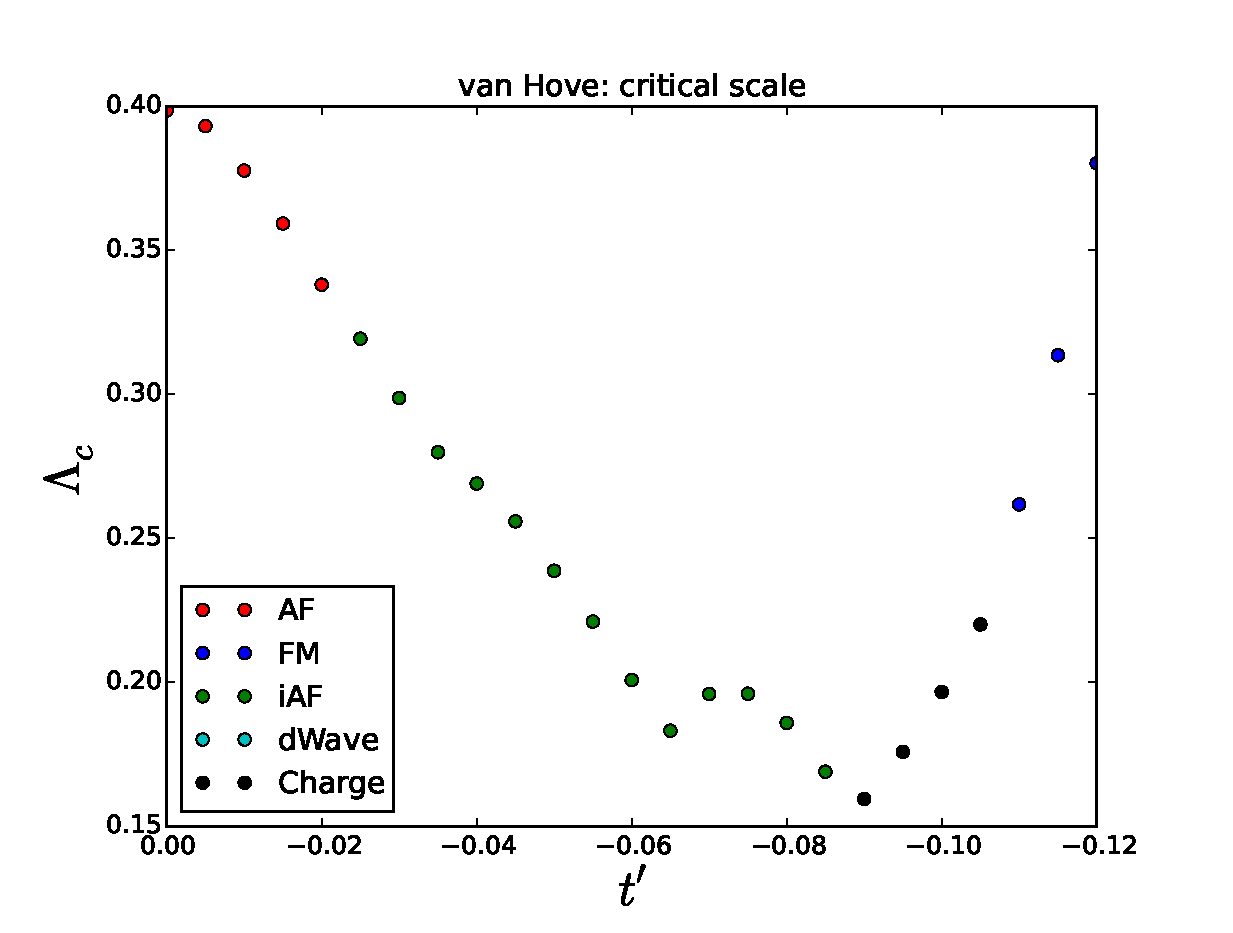
\includegraphics[scale=0.5]{vanHove_scan_critical_lambda_phi.eps}
\caption{Diagrammatic elements used in the text. The Yukawa coupling already refers to the case of spin boson. For a density boson there is a plus sign. } \label{dictionary}

\end{figure}
